\documentclass{article}
\usepackage{amsmath}
\usepackage{graphicx}
\usepackage{geometry}
\usepackage{caption}
\usepackage{tikz}
\usepackage{float}
\usepackage{hyperref}
\usepackage{minted}
\usepackage[backend=biber, style=authoryear]{biblatex}

\geometry{margin=1in}

\title{Understanding the U-Net Architecture with Code}
\author{}
\date{}

\addbibresource{references.bib}

\begin{document}

\maketitle

The U-Net is made up of contracting path (downsampling), bottleneck (middle part) and expansive path (upsampling).

\begin{figure}[H]
    \centering
    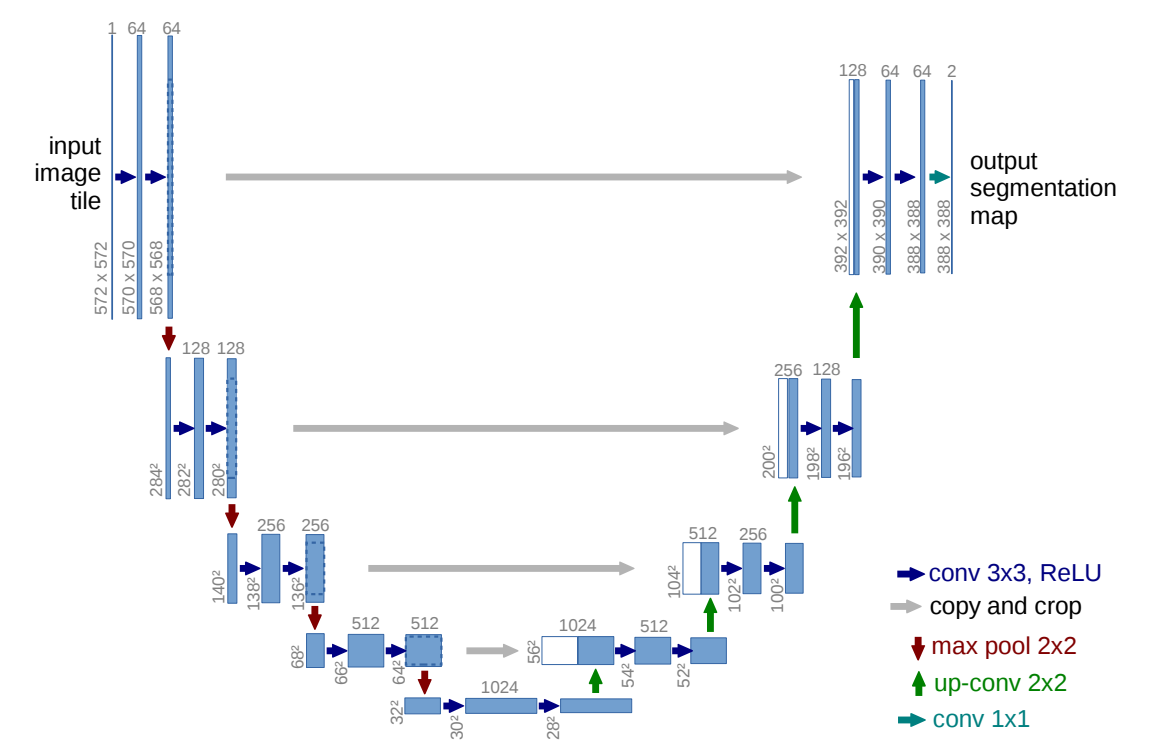
\includegraphics[width=0.8\textwidth]{unet.png}
    \caption{U-Net Architecture}
    \label{fig:unet}
\end{figure}

\tableofcontents
\newpage

\section{Contracting Path (Downsampling)}

The contracting path captures the context of the input image by applying repeated convolution and pooling operations. Each step in the contracting path contains:

\begin{itemize}
    \item \textbf{\textcolor{blue}{Blue arrow}}: Two $3 \times 3$ convolutional layers (with ReLU activation after each convolution layer).
    \item \textbf{\textcolor{red}{Red arrow}}: A $2 \times 2$ max pooling layer with stride 2 for downsampling.
\end{itemize}





\subsection{Blue arrow: Convolutional Block}

\begin{figure}[H]
    \centering
    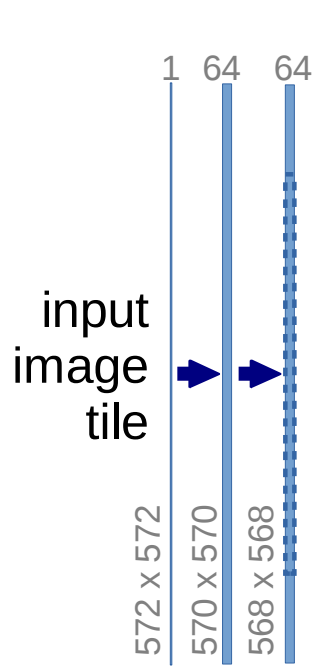
\includegraphics[width=0.15\textwidth]{latex/blue_arrow.png}
    \caption{Double Convolutional Block}
\end{figure}

The double convolution block can be defined as:

\begin{minted}[fontsize=\small, linenos]{python}
class DoubleConvolution(nn.Module):
    def __init__(self, in_channels, out_channels):
        super().__init__()
        self.conv_block = nn.Sequential(
            nn.Conv2d(in_channels, out_channels, kernel_size=3, padding=1),
            nn.ReLU(inplace=True),
            nn.Conv2d(out_channels, out_channels, kernel_size=3, padding=1),
            nn.ReLU(inplace=True)
        )
    
    def forward(self, x):
        return self.conv_block(x)
\end{minted}

Explanation of the code:

\begin{itemize}
    \item The padding of 1 ensures that the spatial dimensions remain the same after convolution. Though in the original paper \cite{unet}, there was no padding; we can see this in figure \ref{fig:unet} where we go from $572 \times 572$ to $570 \times 570$ by the first convolution with kernel size $3 \times 3$, which makes sense.
    
    \item The \texttt{inplace=True} argument in ReLU allows for memory optimization by modifying the input directly (instead of allocating memory).
\end{itemize}







\subsection{Red arrow: Maxpooling}

The downsampling operation can be implemented as:

\begin{minted}[fontsize=\small, linenos]{python}
class DownSampling(nn.Module):
    def __init__(self, in_channels, out_channels):
        super().__init__()
        self.conv = DoubleConvolution(in_channels, out_channels)
        self.pool = nn.MaxPool2d(kernel_size=2, stride=2)
    
    def forward(self, x):
        down = self.conv(x)
        pool = self.pool(down)

        return down, pool
\end{minted}

% TODO: Explain why we have two outputs
Explanation of the code:

\begin{itemize}
    \item The \texttt{down} feature map is retained for later use in skip connections.
    \item The \texttt{pool} is forwarded deeper into the network.
\end{itemize}











\section{Bottleneck}

At the bottom of the U, the network contains two $3 \times 3$ convolutions without pooling. This stage learns the most abstract features before upsampling begins.

\section*{3. Expansive Path (Upsampling)}

The expansive path reconstructs the segmentation map through upsampling and concatenation with features from the contracting path. Each step includes:
\begin{itemize}
    \item A $2 \times 2$ transposed convolution for upsampling.
    \item Concatenation with the corresponding feature map from the contracting path.
    \item Two $3 \times 3$ convolutions (with ReLU activation).
\end{itemize}

The implementation of an upsampling block:

\begin{verbatim}
class UpSampling(nn.Module):
    def __init__(self, in_channels, out_channels):
        self.up = nn.ConvTranspose2d(in_channels, in_channels // 2, kernel_size=2, stride=2)
        self.conv = DoubleConvolution(in_channels, out_channels)

    def forward(self, x1, x2):
        x1 = self.up(x1)
        x = torch.cat((x1, x2), dim=1)
        return self.conv(x)
\end{verbatim}

\section*{4. Skip Connections}

Skip connections play a critical role in U-Net. They allow high-resolution features from the encoder to be reused in the decoder, which helps retain fine-grained spatial information lost during pooling. They are implemented by concatenating encoder features with the decoder's upsampled output:

\begin{equation}
x = \text{Concat}(\text{Upsample}(x_{\text{decoder}}), x_{\text{encoder}})
\end{equation}

This helps the network make better predictions, especially near object boundaries.

\section*{5. Final Output}

The final layer is typically a $1 \times 1$ convolution to reduce the number of feature maps to the number of classes in the segmentation task.

\begin{verbatim}
self.out = nn.Conv2d(64, num_classes, kernel_size=1)
\end{verbatim}

\section*{Conclusion}

U-Net's strength lies in its symmetric structure and use of skip connections. This design enables the network to combine both high-level abstract features and low-level spatial information, making it highly effective for segmentation tasks with limited data.

\end{document}
